\section*{5. Results Summary}

% ------------------------------------------------------------------
\subsection*{Exp-6a: 4-bit Adder (CD4008)}
The expected outputs are calculated from $A + B + C_1$. An LED that is on means logic 1.

\begin{table}[H]
\centering
\small
\begin{tabular}{c | c c c | c c c | c c}
\toprule
\multirow{2}{*}{\textbf{Case}} & \multicolumn{3}{c|}{\textbf{Inputs}} & \multicolumn{3}{c|}{\textbf{Expected}} & \multicolumn{2}{c}{\textbf{Measured}} \\
 & $A_4A_3A_2A_1$ & $B_4B_3B_2B_1$ & $C_1$ & Decimal & $C_O$ & $S_4S_3S_2S_1$ & $C_O$ & $S_4S_3S_2S_1$ \\
\midrule
1 & 0001 & 0101 & 0 & $1 + 5 + 0 = 6$   & 0 & 0110 & 0 & 0110 \\
2 & 1010 & 0101 & 1 & $10 + 5 + 1 = 16$ & 1 & 0000 & 1 & 0000 \\
3 & 1100 & 1101 & 0 & $12 + 13 + 0 = 25$ & 1 & 1001 & 1 & 1001 \\
4 & 1111 & 1110 & 1 & $15 + 14 + 1 = 30$ & 1 & 1110 & 1 & 1110 \\
\bottomrule
\end{tabular}
\captionof{table}{CD4008 test cases: expected vs.\ measured outputs}
\label{tab:6a}
\end{table}
For all four cases, the measured $C_O$ and $S_4S_3S_2S_1$ match the expected values.

% TODO: 確認照片順序 IMG_7087~7090 是否對應 Case 1~4
\begin{figure}[H]
    \centering
    \begin{minipage}[t]{0.48\textwidth}
        \centering
        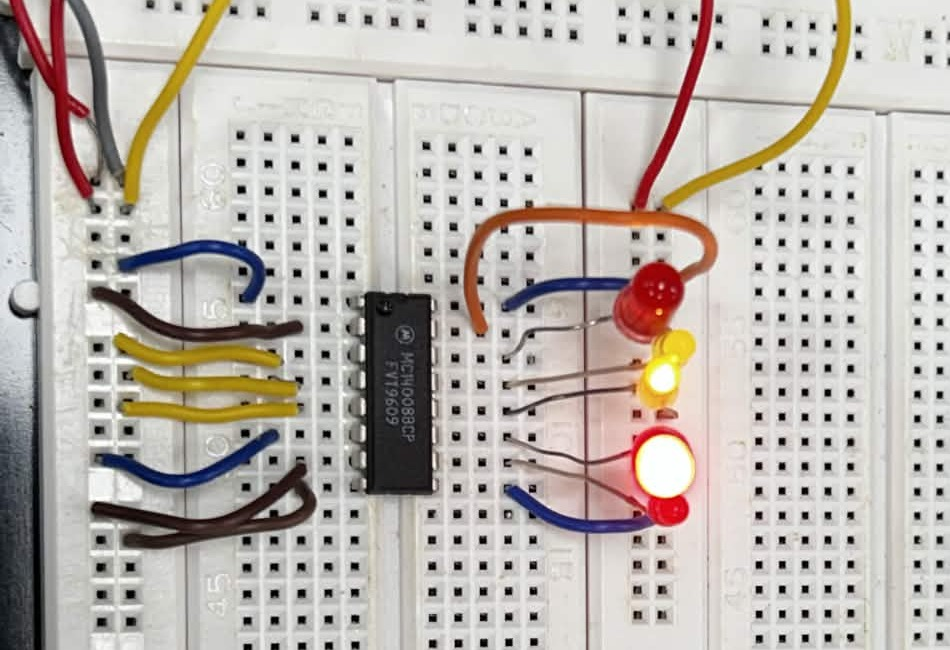
\includegraphics[width=\linewidth]{pic/adder_1.jpg}
        \captionof{figure}{Case 1: $0001 + 0101$, $C_1 = 0$}
        \label{fig:6a_case1}
    \end{minipage}
    \hfill
    \begin{minipage}[t]{0.48\textwidth}
        \centering
        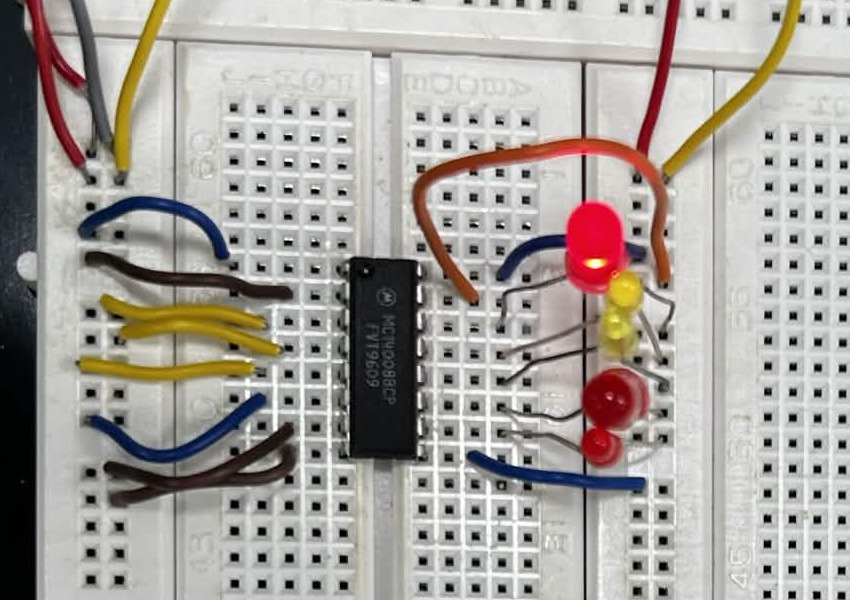
\includegraphics[width=\linewidth]{pic/adder_2.jpg}
        \captionof{figure}{Case 2: $1010 + 0101$, $C_1 = 1$}
        \label{fig:6a_case2}
    \end{minipage}

    \vspace{0.5em}
    \begin{minipage}[t]{0.48\textwidth}
        \centering
        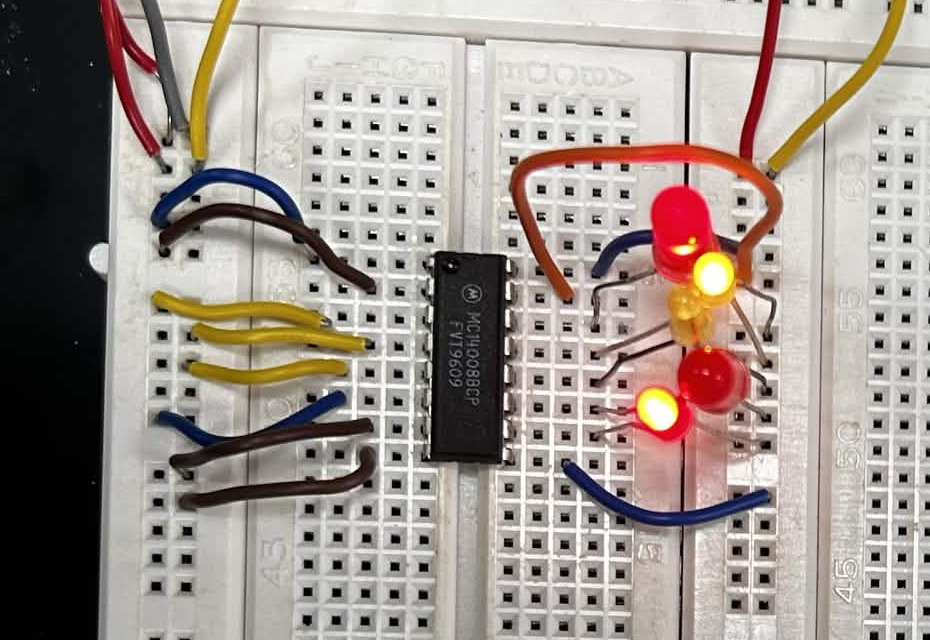
\includegraphics[width=\linewidth]{pic/adder_3.jpg}
        \captionof{figure}{Case 3: $1100 + 1101$, $C_1 = 0$}
        \label{fig:6a_case3}
    \end{minipage}
    \hfill
    \begin{minipage}[t]{0.48\textwidth}
        \centering
        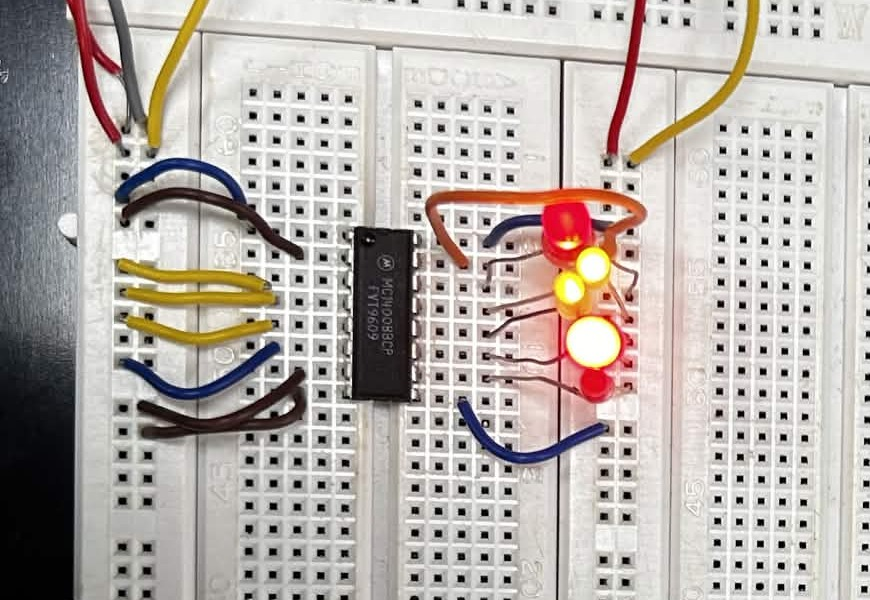
\includegraphics[width=\linewidth]{pic/adder_4.jpg}
        \captionof{figure}{Case 4: $1111 + 1110$, $C_1 = 1$}
        \label{fig:6a_case4}
    \end{minipage}
\end{figure}

\newpage
% ------------------------------------------------------------------
\subsection*{Exp-6b: BCD to 7-Segment Display (CD4511)}
\begin{figure}[H]
    \centering
    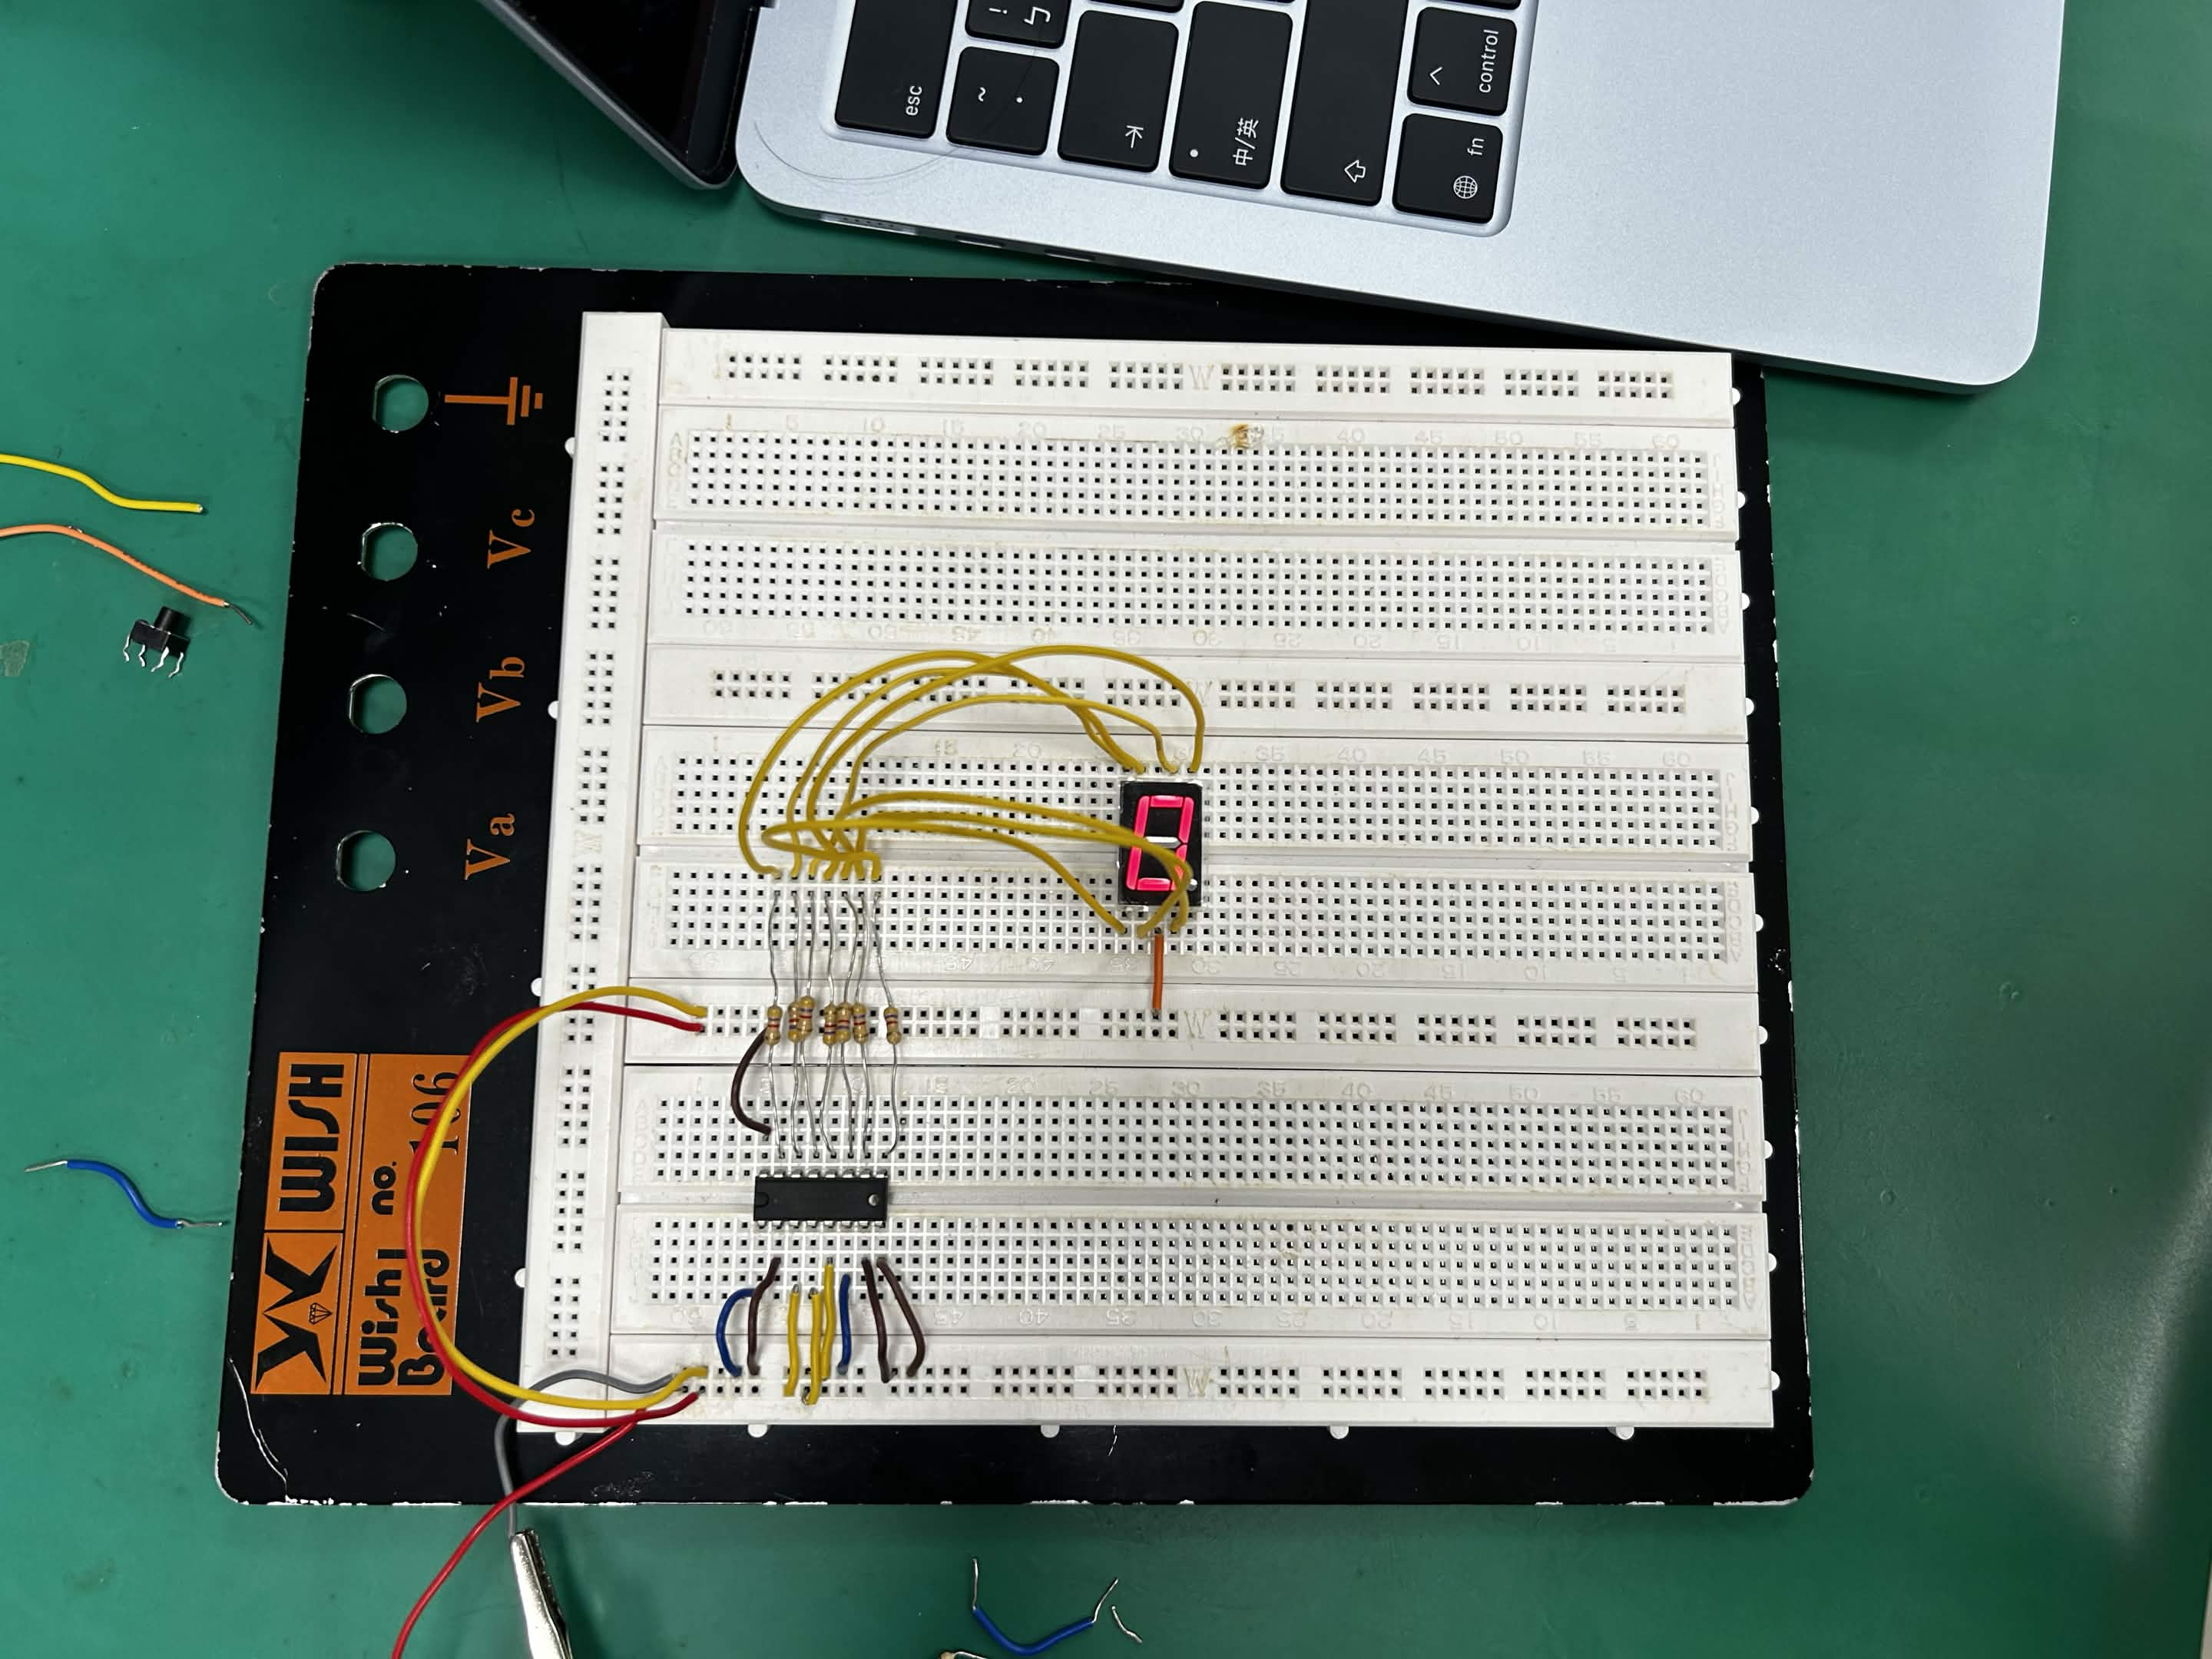
\includegraphics[width=0.75\textwidth]{pic/IMG_7077.jpg}
    \captionof{figure}{Breadboard of Exp-6b (input $0000$, displaying 0)}
    \label{fig:6b_board}
\end{figure}

% 每張照片已裁成只含顯示器的區域：pic/disp_N.jpg（原圖 IMG_7077~7086，7086 為直拍已轉正）
\newcommand{\digitpic}[2]{%
    \begin{minipage}[t]{0.185\textwidth}
        \centering
        \includegraphics[width=\linewidth]{pic/disp_#1.jpg}\\[2pt]
        \small #1 ($#2$)
    \end{minipage}}
\begin{figure}[H]
    \centering
    \digitpic{0}{0000}\hfill\digitpic{1}{0001}\hfill\digitpic{2}{0010}\hfill\digitpic{3}{0011}\hfill\digitpic{4}{0100}

    \vspace{0.8em}
    \digitpic{5}{0101}\hfill\digitpic{6}{0110}\hfill\digitpic{7}{0111}\hfill\digitpic{8}{1000}\hfill\digitpic{9}{1001}
    \captionof{figure}{Displayed digits 0--9 with BCD input $DCBA$}
    \label{fig:6b_digits}
\end{figure}

All ten BCD inputs $0000 \sim 1001$ were displayed as the digits 0 to 9, which agrees with the CD4511 truth table (Table~\ref{tab:cd4511}).
